\hypertarget{framehelpers_8h}{
\section{framehelpers.h File Reference}
\label{framehelpers_8h}\index{framehelpers.h@{framehelpers.h}}
}
Helpfunctions for programs that have to deal with Frames. 

{\tt \#include $<$linux/types.h$>$}\par


Include dependency graph for framehelpers.h:\begin{figure}[H]
\begin{center}
\leavevmode
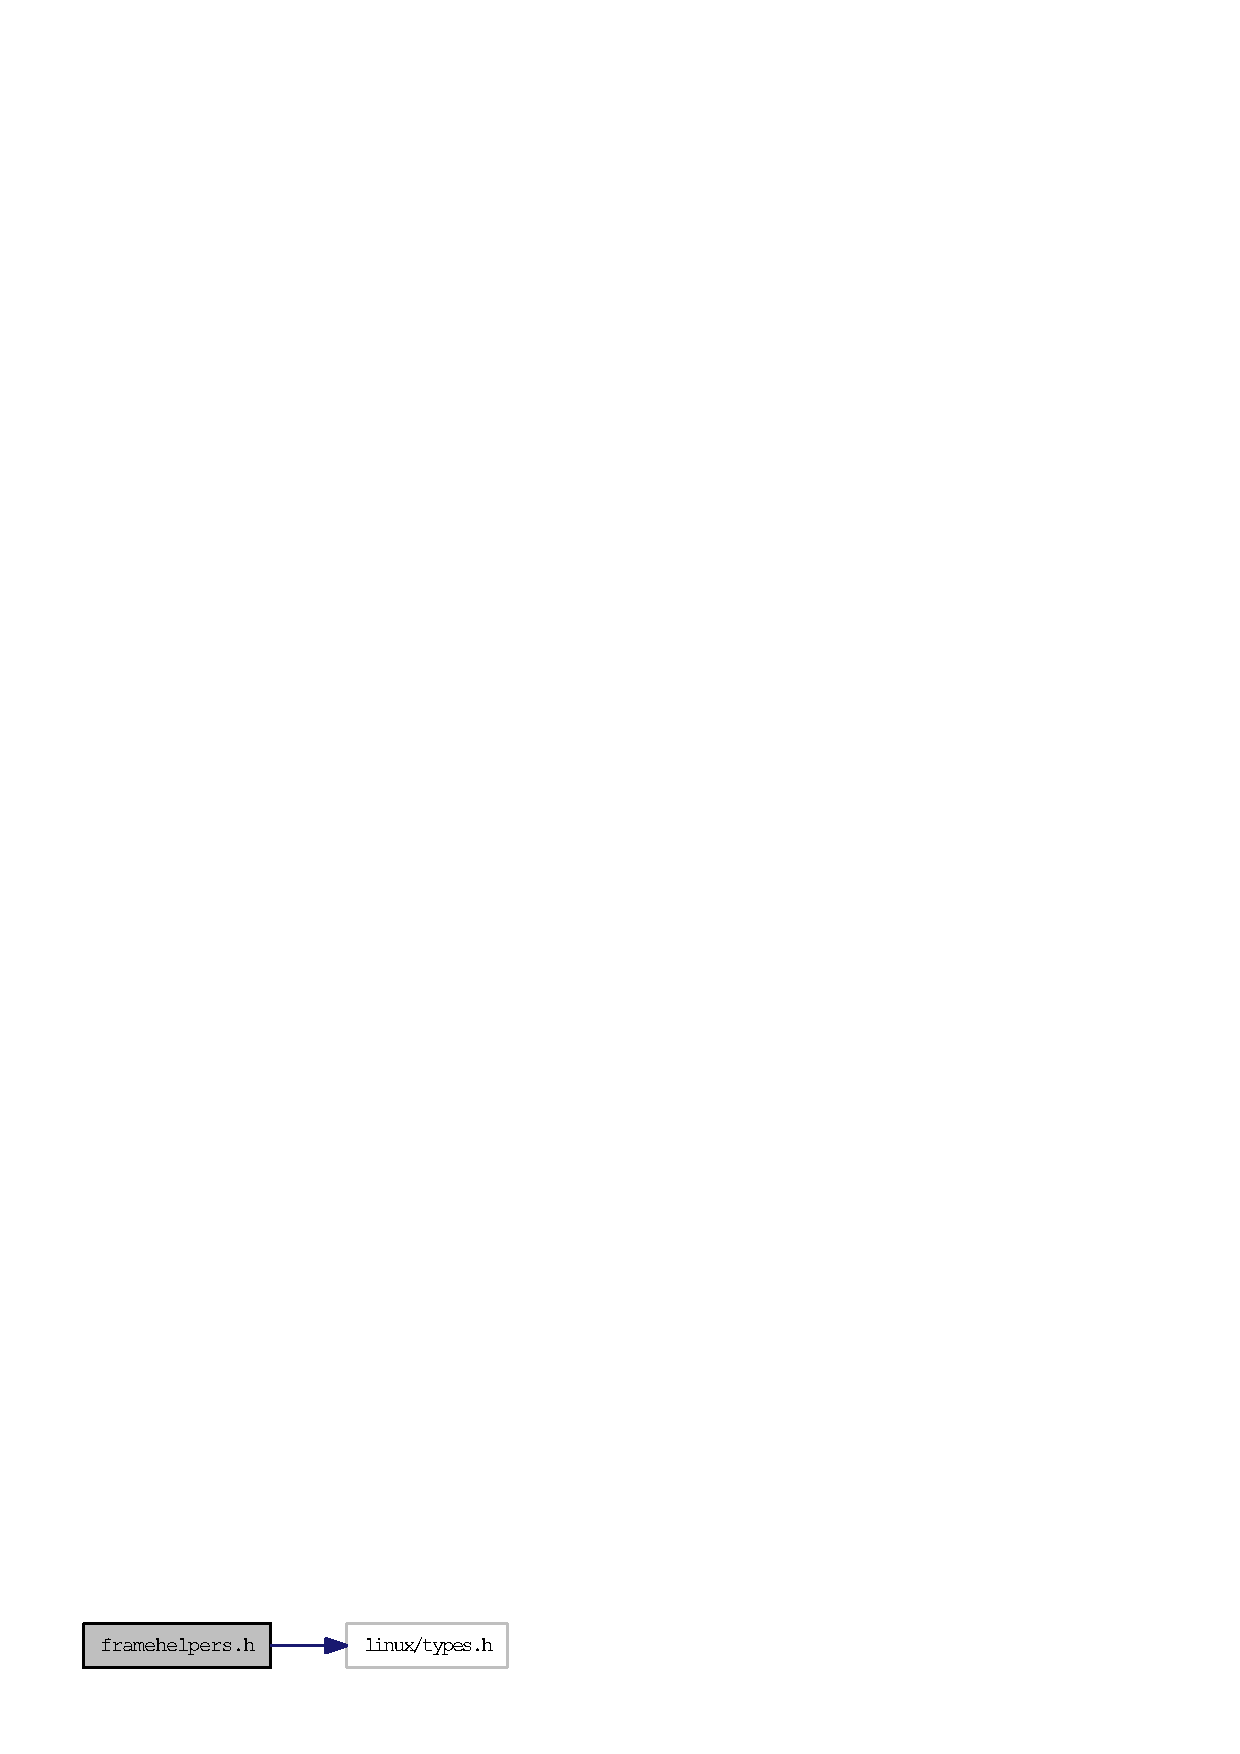
\includegraphics[width=124pt]{framehelpers_8h__incl}
\end{center}
\end{figure}


This graph shows which files directly or indirectly include this file:\begin{figure}[H]
\begin{center}
\leavevmode
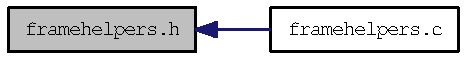
\includegraphics[width=130pt]{framehelpers_8h__dep__incl}
\end{center}
\end{figure}
\subsection*{Functions}
\begin{CompactItemize}
\item 
\_\-\_\-u16 \hyperlink{framehelpers_8h_ec06976aa28c099e56494e715860844b}{get\-Upper\-Address} (\_\-\_\-u32 u32address)
\begin{CompactList}\small\item\em The bits 16 to 31 from an 32 bit address are returned as an 16 bit address. \item\end{CompactList}\item 
\_\-\_\-u16 \hyperlink{framehelpers_8h_045a12bd4874a62c6ed9e9f3ced0c480}{get\-Lower\-Address} (\_\-\_\-u32 u32address)
\begin{CompactList}\small\item\em The bits 0 to 15 from an 32 bit address are returned as an 16 bit address. \item\end{CompactList}\item 
int \hyperlink{framehelpers_8h_019759de9c99bad88139a7ca43d05315}{get\-File\-Size} (char $\ast$path)
\begin{CompactList}\small\item\em checks the filesize of a file with the given path \item\end{CompactList}\item 
int \hyperlink{framehelpers_8h_cd171ecc285f52f3d632227fff34b6fc}{calculate\-Stop\-Address} (int filesize, int startaddress)
\begin{CompactList}\small\item\em calculates the stop address for initial config and scrubbing after the formula: stopaddress = (startaddress + (filesize / 2) - 1) if the firmware has the version 1.2 then 0x100h is added to the stopaddress. \item\end{CompactList}\item 
int \hyperlink{framehelpers_8h_527bff0bf2cd2780c8d0bbe5658c7e71}{enter\-Flash\-State} (int oldstate)
\begin{CompactList}\small\item\em if state is different from flash, then the flash state will be entered. \item\end{CompactList}\item 
int \hyperlink{framehelpers_8h_2ff76e903eb4ccb3b086b6d1d2e895c0}{get\-Bus\-State} ()
\begin{CompactList}\small\item\em checks the state of the RCU BUS and returns this state \item\end{CompactList}\item 
int \hyperlink{framehelpers_8h_1b593ec8f8b80418b87f3d9da5d6935a}{restore\-Bus\-State} (int oldstate)
\begin{CompactList}\small\item\em If the oldstate was something different then flash, restore\-Bus\-State switches back to this state. \item\end{CompactList}\item 
int \hyperlink{framehelpers_8h_53be595c1a44f646523cdd1f89a0a8a2}{get\-Frame\-Address\-From\-Line} (char line\mbox{[}255\mbox{]}, int $\ast$pframeaddr)
\begin{CompactList}\small\item\em takes a line from the frames file and extracts the frame numbers block, major and minor and write them in the 3 element int array pointed to by the pointer pframeaddr. \item\end{CompactList}\item 
int \hyperlink{framehelpers_8h_8bc9e8e93d38aa4c254464aa672690df}{char\-To\-Int} (char zeichen)
\begin{CompactList}\small\item\em very propably useless - check that later reads an character and returns an int \item\end{CompactList}\item 
int \hyperlink{framehelpers_8h_670a3ae7cf5d6c4357b52b7d756a1434}{get\-Linesnumber\-From\-File} (char $\ast$filename)
\begin{CompactList}\small\item\em used for reading the framesfile \item\end{CompactList}\item 
int \hyperlink{framehelpers_8h_e0753d753c40cd8d8de955f40968d272}{get\-Hex\-Value\-From\-Line} (char line\mbox{[}255\mbox{]}, unsigned short $\ast$p\-Addresses)
\begin{CompactList}\small\item\em used for reading the header and footer files. \item\end{CompactList}\end{CompactItemize}


\subsection{Detailed Description}
Helpfunctions for programs that have to deal with Frames. 

\begin{Desc}
\item[Author:]Dominik Fehlker \end{Desc}
\begin{Desc}
\item[Date:]\end{Desc}


Definition in file \hyperlink{framehelpers_8h-source}{framehelpers.h}.

\subsection{Function Documentation}
\hypertarget{framehelpers_8h_cd171ecc285f52f3d632227fff34b6fc}{
\index{framehelpers.h@{framehelpers.h}!calculateStopAddress@{calculateStopAddress}}
\index{calculateStopAddress@{calculateStopAddress}!framehelpers.h@{framehelpers.h}}
\subsubsection[calculateStopAddress]{\setlength{\rightskip}{0pt plus 5cm}int calculate\-Stop\-Address (int {\em filesize}, int {\em startaddress})}}
\label{framehelpers_8h_cd171ecc285f52f3d632227fff34b6fc}


calculates the stop address for initial config and scrubbing after the formula: stopaddress = (startaddress + (filesize / 2) - 1) if the firmware has the version 1.2 then 0x100h is added to the stopaddress. 

\begin{Desc}
\item[Parameters:]
\begin{description}
\item[{\em filesize}]the filesize of the framefile to program \item[{\em startaddress}]the startaddress where programming has begun \end{description}
\end{Desc}
\begin{Desc}
\item[Returns:]the stopaddress \end{Desc}


Definition at line 78 of file framehelpers.c.

References e\-Enable\-Flash, e\-Enable\-Msg\-Buf, EXIT\_\-FAILURE, rcu\-Bus\-Control\-Cmd(), and rcu\-Single\-Read().

Referenced by do\-Init(), and do\-Scrubbing().

Here is the call graph for this function:\begin{figure}[H]
\begin{center}
\leavevmode
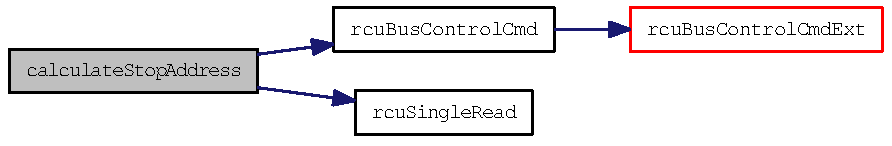
\includegraphics[width=232pt]{framehelpers_8h_cd171ecc285f52f3d632227fff34b6fc_cgraph}
\end{center}
\end{figure}
\hypertarget{framehelpers_8h_8bc9e8e93d38aa4c254464aa672690df}{
\index{framehelpers.h@{framehelpers.h}!charToInt@{charToInt}}
\index{charToInt@{charToInt}!framehelpers.h@{framehelpers.h}}
\subsubsection[charToInt]{\setlength{\rightskip}{0pt plus 5cm}int char\-To\-Int (char {\em zeichen})}}
\label{framehelpers_8h_8bc9e8e93d38aa4c254464aa672690df}


very propably useless - check that later reads an character and returns an int 

\begin{Desc}
\item[Returns:]the integer value according to the character, everything else than 0-9 returns -1 \end{Desc}


Definition at line 279 of file framehelpers.c.\hypertarget{framehelpers_8h_527bff0bf2cd2780c8d0bbe5658c7e71}{
\index{framehelpers.h@{framehelpers.h}!enterFlashState@{enterFlashState}}
\index{enterFlashState@{enterFlashState}!framehelpers.h@{framehelpers.h}}
\subsubsection[enterFlashState]{\setlength{\rightskip}{0pt plus 5cm}int enter\-Flash\-State (int {\em oldstate})}}
\label{framehelpers_8h_527bff0bf2cd2780c8d0bbe5658c7e71}


if state is different from flash, then the flash state will be entered. 

\begin{Desc}
\item[Parameters:]
\begin{description}
\item[{\em oldstate}]the state before entering flash state \end{description}
\end{Desc}
\begin{Desc}
\item[Returns:]not used \end{Desc}


Definition at line 115 of file framehelpers.c.

References e\-Enable\-Flash, e\-Enable\-Msg\-Buf, and rcu\-Bus\-Control\-Cmd().

Referenced by main().

Here is the call graph for this function:\begin{figure}[H]
\begin{center}
\leavevmode
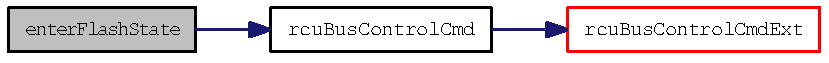
\includegraphics[width=217pt]{framehelpers_8h_527bff0bf2cd2780c8d0bbe5658c7e71_cgraph}
\end{center}
\end{figure}
\hypertarget{framehelpers_8h_2ff76e903eb4ccb3b086b6d1d2e895c0}{
\index{framehelpers.h@{framehelpers.h}!getBusState@{getBusState}}
\index{getBusState@{getBusState}!framehelpers.h@{framehelpers.h}}
\subsubsection[getBusState]{\setlength{\rightskip}{0pt plus 5cm}int get\-Bus\-State ()}}
\label{framehelpers_8h_2ff76e903eb4ccb3b086b6d1d2e895c0}


checks the state of the RCU BUS and returns this state 

\begin{Desc}
\item[Returns:]the current state of the RCU Bus (1 means selectmap, 2 flash and 3 Msg\-Buffer) \end{Desc}


Definition at line 143 of file framehelpers.c.

References e\-Check\-Flash, e\-Check\-Msg\-Buf, e\-Check\-Selectmap, and rcu\-Bus\-Control\-Cmd().

Referenced by main().

Here is the call graph for this function:\begin{figure}[H]
\begin{center}
\leavevmode
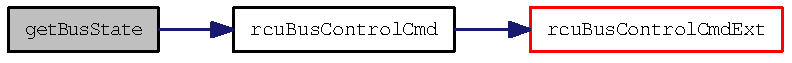
\includegraphics[width=208pt]{framehelpers_8h_2ff76e903eb4ccb3b086b6d1d2e895c0_cgraph}
\end{center}
\end{figure}
\hypertarget{framehelpers_8h_019759de9c99bad88139a7ca43d05315}{
\index{framehelpers.h@{framehelpers.h}!getFileSize@{getFileSize}}
\index{getFileSize@{getFileSize}!framehelpers.h@{framehelpers.h}}
\subsubsection[getFileSize]{\setlength{\rightskip}{0pt plus 5cm}int get\-File\-Size (char $\ast$ {\em path})}}
\label{framehelpers_8h_019759de9c99bad88139a7ca43d05315}


checks the filesize of a file with the given path 

\begin{Desc}
\item[Returns:]the filesize in Bytes \end{Desc}


Definition at line 88 of file bitswapper.c.

References EXIT\_\-FAILURE.\hypertarget{framehelpers_8h_53be595c1a44f646523cdd1f89a0a8a2}{
\index{framehelpers.h@{framehelpers.h}!getFrameAddressFromLine@{getFrameAddressFromLine}}
\index{getFrameAddressFromLine@{getFrameAddressFromLine}!framehelpers.h@{framehelpers.h}}
\subsubsection[getFrameAddressFromLine]{\setlength{\rightskip}{0pt plus 5cm}int get\-Frame\-Address\-From\-Line (char {\em line}\mbox{[}255\mbox{]}, int $\ast$ {\em pframeaddr})}}
\label{framehelpers_8h_53be595c1a44f646523cdd1f89a0a8a2}


takes a line from the frames file and extracts the frame numbers block, major and minor and write them in the 3 element int array pointed to by the pointer pframeaddr. 

In case something not useful is read, block, major and minor are -1

\begin{Desc}
\item[Parameters:]
\begin{description}
\item[{\em line}]a line to be fragmented \item[{\em $\ast$pframaddr}]the 3 element int array which holds block, major and minor \end{description}
\end{Desc}


Definition at line 200 of file framehelpers.c.

References char\-To\-Int().

Referenced by do\-Flash\-Frame(), get\-Linesnumber\-From\-File(), and main().

Here is the call graph for this function:\begin{figure}[H]
\begin{center}
\leavevmode
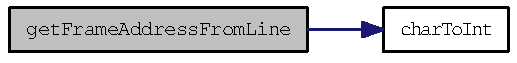
\includegraphics[width=142pt]{framehelpers_8h_53be595c1a44f646523cdd1f89a0a8a2_cgraph}
\end{center}
\end{figure}
\hypertarget{framehelpers_8h_e0753d753c40cd8d8de955f40968d272}{
\index{framehelpers.h@{framehelpers.h}!getHexValueFromLine@{getHexValueFromLine}}
\index{getHexValueFromLine@{getHexValueFromLine}!framehelpers.h@{framehelpers.h}}
\subsubsection[getHexValueFromLine]{\setlength{\rightskip}{0pt plus 5cm}int get\-Hex\-Value\-From\-Line (char {\em line}\mbox{[}255\mbox{]}, unsigned short $\ast$ {\em p\-Addresses})}}
\label{framehelpers_8h_e0753d753c40cd8d8de955f40968d272}


used for reading the header and footer files. 

reads a 4 digit hex value from the given char array if it finds the variables \char`\"{}\$frame\_\-addr31\_\-16\char`\"{} or \char`\"{}\$frame\_\-addr15\_\-0\char`\"{} the address values from the given unsigned short array with two elements is used.

\begin{Desc}
\item[Parameters:]
\begin{description}
\item[{\em line}]the line where the hex value shall be read from \item[{\em p\-Addresses}]the 2 element unsigned short array which holds add31\_\-16 and addr15\_\-0 \end{description}
\end{Desc}
\begin{Desc}
\item[Returns:]the hexadecimal value \end{Desc}


Definition at line 339 of file framehelpers.c.

Referenced by main().\hypertarget{framehelpers_8h_670a3ae7cf5d6c4357b52b7d756a1434}{
\index{framehelpers.h@{framehelpers.h}!getLinesnumberFromFile@{getLinesnumberFromFile}}
\index{getLinesnumberFromFile@{getLinesnumberFromFile}!framehelpers.h@{framehelpers.h}}
\subsubsection[getLinesnumberFromFile]{\setlength{\rightskip}{0pt plus 5cm}int get\-Linesnumber\-From\-File (char $\ast$ {\em filename})}}
\label{framehelpers_8h_670a3ae7cf5d6c4357b52b7d756a1434}


used for reading the framesfile 

takes an character array with up to 255 characters and seperates them using \char`\"{};\char`\"{} into Block-, Major- and Minornumber. Calculates the address31\_\-16 and address15\_\-0 for the globale variables as well as the w\_\-frame\-X.X.X.hex and r\_\-frame.X.X.X.hex filenames. Example line for frames.txt: 0;5;3;

comments can be made using a leading \char`\"{}\#\char`\"{} 

Definition at line 308 of file framehelpers.c.

References EXIT\_\-FAILURE, and get\-Frame\-Address\-From\-Line().

Referenced by do\-Flash\-Frame(), and main().

Here is the call graph for this function:\begin{figure}[H]
\begin{center}
\leavevmode
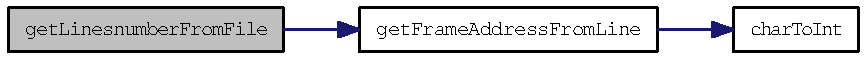
\includegraphics[width=226pt]{framehelpers_8h_670a3ae7cf5d6c4357b52b7d756a1434_cgraph}
\end{center}
\end{figure}
\hypertarget{framehelpers_8h_045a12bd4874a62c6ed9e9f3ced0c480}{
\index{framehelpers.h@{framehelpers.h}!getLowerAddress@{getLowerAddress}}
\index{getLowerAddress@{getLowerAddress}!framehelpers.h@{framehelpers.h}}
\subsubsection[getLowerAddress]{\setlength{\rightskip}{0pt plus 5cm}\_\-\_\-u16 get\-Lower\-Address (\_\-\_\-u32 {\em u32address})}}
\label{framehelpers_8h_045a12bd4874a62c6ed9e9f3ced0c480}


The bits 0 to 15 from an 32 bit address are returned as an 16 bit address. 

\begin{Desc}
\item[Returns:]the lower 16 bits (0 to 15) \end{Desc}


Definition at line 45 of file framehelpers.c.

Referenced by do\-Flash\-Frame(), do\-Init(), and do\-Scrubbing().\hypertarget{framehelpers_8h_ec06976aa28c099e56494e715860844b}{
\index{framehelpers.h@{framehelpers.h}!getUpperAddress@{getUpperAddress}}
\index{getUpperAddress@{getUpperAddress}!framehelpers.h@{framehelpers.h}}
\subsubsection[getUpperAddress]{\setlength{\rightskip}{0pt plus 5cm}\_\-\_\-u16 get\-Upper\-Address (\_\-\_\-u32 {\em u32address})}}
\label{framehelpers_8h_ec06976aa28c099e56494e715860844b}


The bits 16 to 31 from an 32 bit address are returned as an 16 bit address. 

\begin{Desc}
\item[Returns:]the upper 16 Bits (16 to 31) \end{Desc}


Definition at line 34 of file framehelpers.c.

Referenced by do\-Flash\-Frame(), do\-Init(), and do\-Scrubbing().\hypertarget{framehelpers_8h_1b593ec8f8b80418b87f3d9da5d6935a}{
\index{framehelpers.h@{framehelpers.h}!restoreBusState@{restoreBusState}}
\index{restoreBusState@{restoreBusState}!framehelpers.h@{framehelpers.h}}
\subsubsection[restoreBusState]{\setlength{\rightskip}{0pt plus 5cm}int restore\-Bus\-State (int {\em oldstate})}}
\label{framehelpers_8h_1b593ec8f8b80418b87f3d9da5d6935a}


If the oldstate was something different then flash, restore\-Bus\-State switches back to this state. 

if oldstate was already flash, then nothing is done.

\begin{Desc}
\item[Parameters:]
\begin{description}
\item[{\em oldstate}]the old state of the Bus \end{description}
\end{Desc}
\begin{Desc}
\item[Returns:]not used \end{Desc}


Definition at line 165 of file framehelpers.c.

References e\-Enable\-Msg\-Buf, e\-Enable\-Selectmap, and rcu\-Bus\-Control\-Cmd().

Referenced by main().

Here is the call graph for this function:\begin{figure}[H]
\begin{center}
\leavevmode
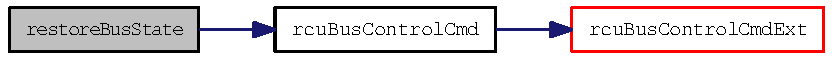
\includegraphics[width=218pt]{framehelpers_8h_1b593ec8f8b80418b87f3d9da5d6935a_cgraph}
\end{center}
\end{figure}
